% vim:ts=4:sw=4
% Copyright (c) 2014 Casper Ti. Vector
% Public domain.

\chapter{绪论}
% 中文测试文字。
\section{研究背景}

高速公路是服务群众生活、支撑国家经济发展、保障国家安全的战略设施和资源。截止2016年底,我国公路通车总里程达到457万公里,其中高速公路12万公里,2017年将新增4500公里,是世界上规模最大的高速公路(如图\ref{gaosugonglu}所示)。 

				\begin{figure}[h]
				\centering
						\begin{minipage}{0.8\linewidth}
							\centering
							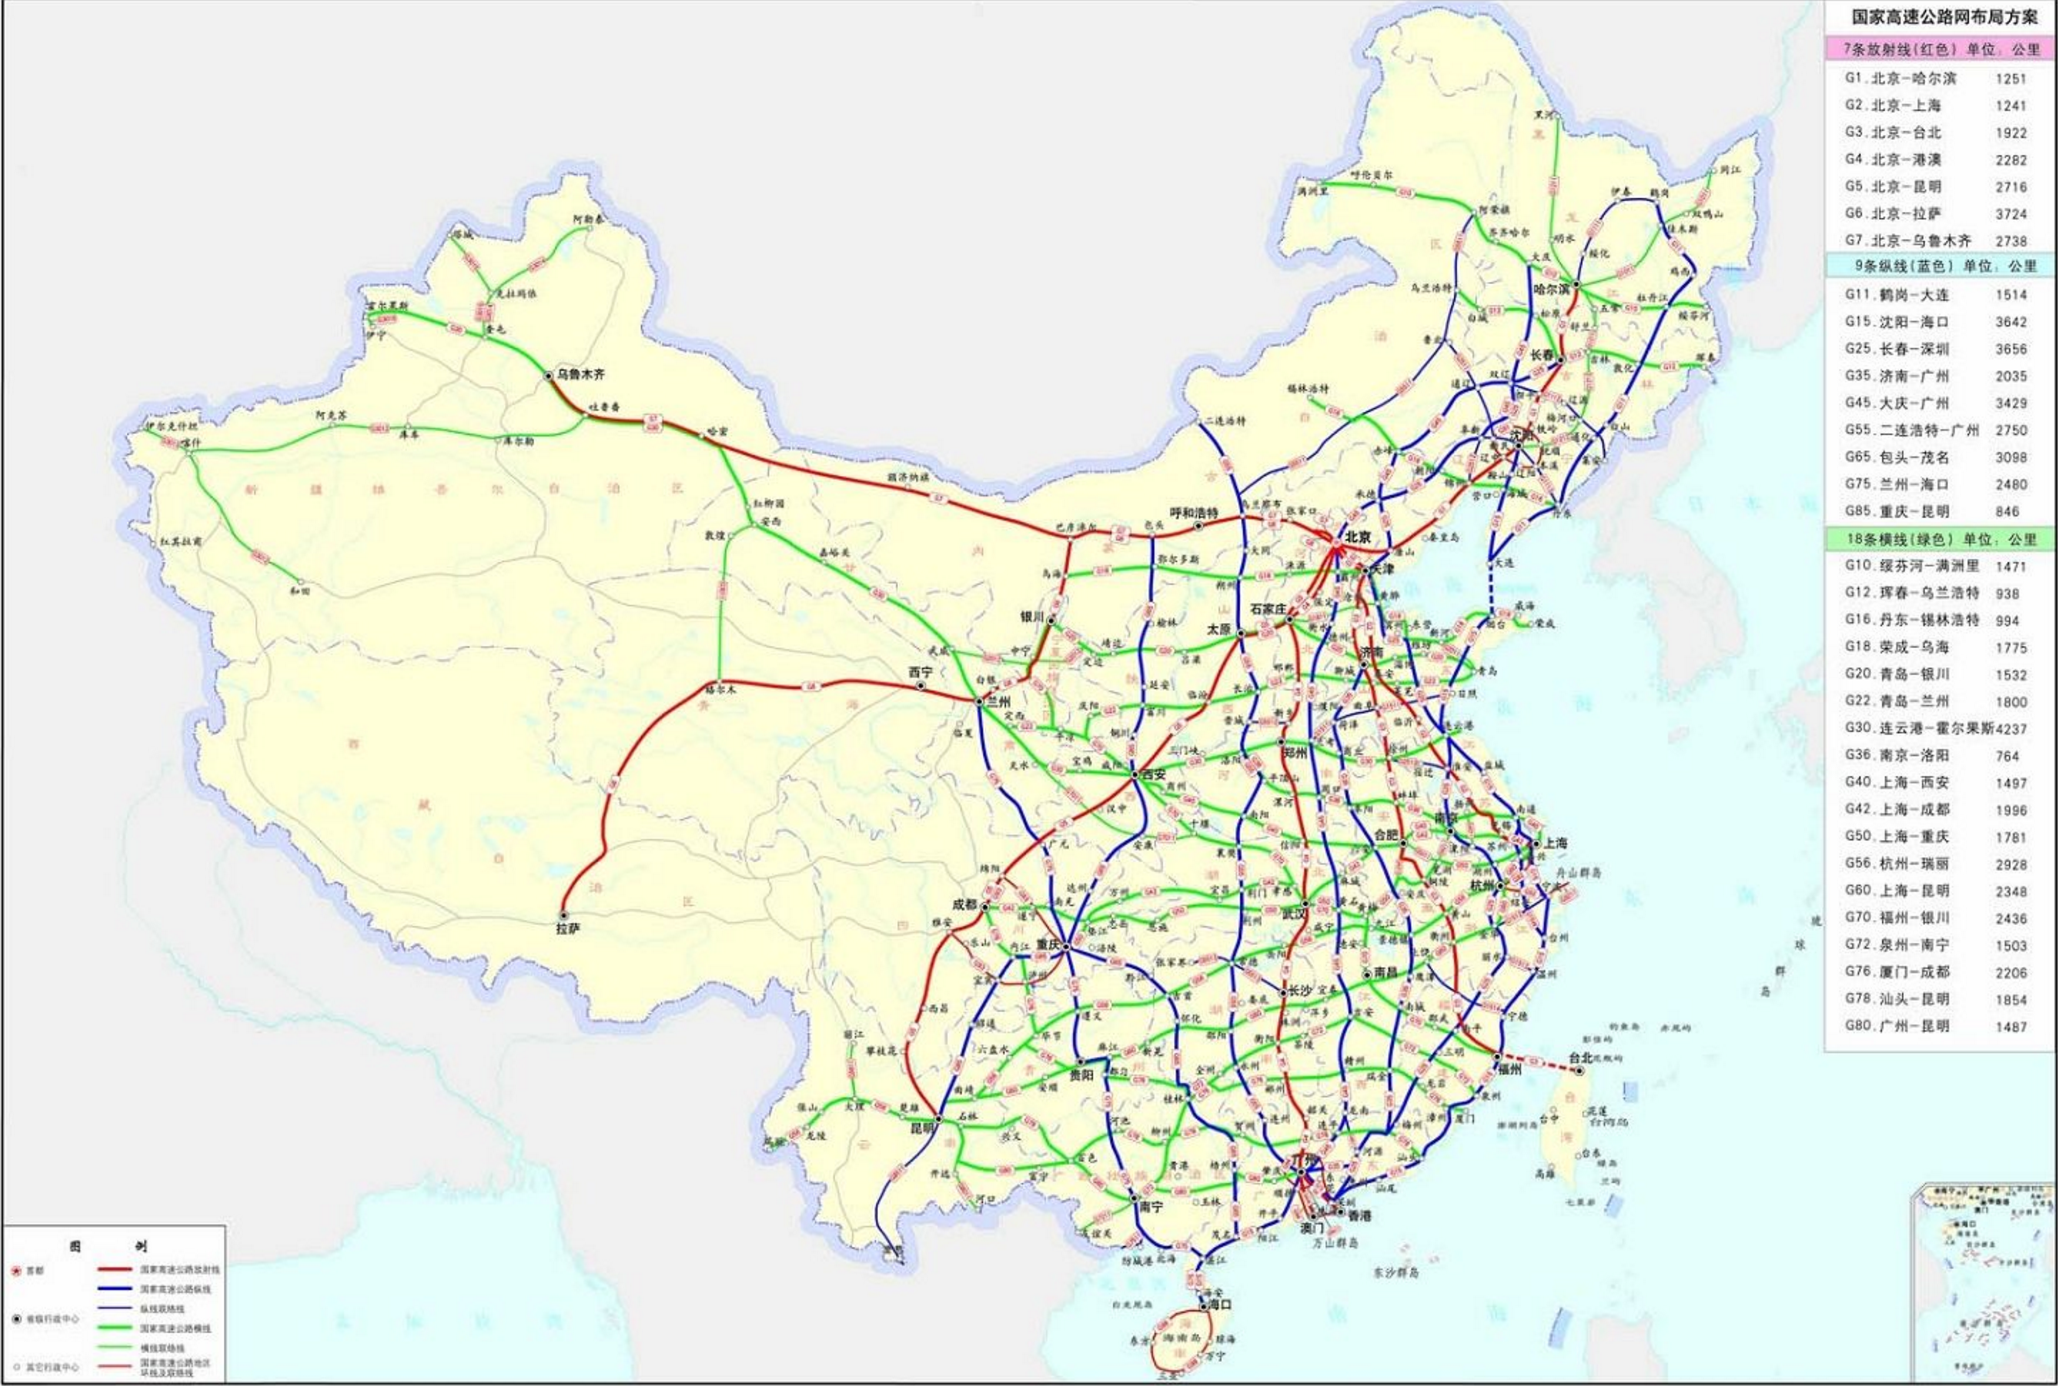
\includegraphics[width=4.4in]{picture/gaosugonglu}
							\caption{中国高速公路网络示意图}
							\label{gaosugonglu}
						\end{minipage}%\
				\end{figure}

随着中国经济的快速发展,人们生活水平的不断提高,居民的出行和货物运输的数量也在逐渐增加。交通出行是人类活动不可缺少的一部分。据估计,每天平均有40\%的人口在路上花费至少1小时。近几年来,人们变得越来越依赖于交通系统,对于交通管理人员来说,机遇和挑战共存。首先,交通拥堵已成为一个日益严重的问题。全球范围内的道路上的车辆增加,根据调查,截止至2016年初,北京共有544万辆车,比2014年初增加了50万辆。这些激增的车辆会对道路系统产生严重的压力,极大的增加拥堵以及拥堵后的损耗。拥堵会导致燃油消耗增加,空气污染,以及实施公共交通计划的困难。车流流量过多时,交通事故风险与交通运输系统中的膨胀增加,交通事故之后的恢复时间与恢复代价也会急剧增加。在中国,2009年的交通事故死亡人数约有7万人,在2015年达到9万人。美国联邦公路管理局公布的报告显示,发生在城市的交通事故约占所有拥堵延误的50\% - 60\%。一个国家的技术竞争力、经济实力和生产能力,在很大程度上取决于其交通系统性能。交通管理资源有限,中国高速公路正在逐渐走向免费通行,难以对交通系统进行全面建设;同时,国家运输系统的有效性也依赖于一个国家的处理紧急情况的能力,如交通事故发生以后的大规模疏散。随着高速公路的不断发展,各类维护高速公路的需求也都被一一提出:

1)人员分配问题。最典型的是今年五一,交通部联合路政大队、高速交警大队、项目部制定组有针对性的应急预案,根据历史的交通信息,负责做好恶劣天气、旅游高峰车流量饱和、突发事件引起交通阻塞的应急处理。安排值班人员,落实机械设备和应急物资准备,一旦发生突发事件,迅速启动,切实做好节日期的保畅工作。

2)安全管理。面对节日期间可能出现的状况,高速公路养护所需要在节日前期组织开展道路安全隐患检查活动:一是对管段路段进行安全隐患排查,发现问题立即落实整改;二是加强春季防火工作的管理,及时清理桥涵构造物下的易燃物品,对边坡、中央分隔带进行打草、苗木修剪,对匝道圈进行专人看护,安排养护员负责所辖路段的防火报警工作。

3)基础设施建设。交通的基础设施建设主要包括交通轨道交通设施建设、停车场设施建设等。交通基础设施包括为交通系统保障安全正常运营而建设的隧道、公路、轨道、通风亭、通信信号、高架道路、车站、供电系统、机电设备、道路标线等设施。

4)高新设施建设。目前越来越多的新技术涌现,高新技术层出不穷\parencite{ysk2017qx}。这些新技术对高速公路稳定性的提高具有重要意义,但是,新技术普遍造价高昂,无法直接大面积使用,需要交通管理者进行合理分配。

上述的交通需求中有一个共性,那就是找出高速公路网络中最重要的路段。针对高速公路中的重要路段,交通管理者可以进行针对性管理。高速公路的变化日新月异,传统的研究方法很难准确的预估关键路段,亟需提出一套适用于大规模路网的高速公路的关键路段挖掘识别系统。在准确识别高速公路关键路段的前提下,我们可以进行有效的人员分配,避免资源浪费;可以针对高危路段进行安全管理,减少事故风险;可以针对核心路段进行基础设施建设,提升高速公路稳定性,节省预算;可以研究道路施工问题,合理分配施工路段,将施工造成的影响减到最小。高速公路关键路段挖掘问题是交通研究领域重要的的基础问题。

本文提出面向高速公路的关键路段挖掘模型,以高速公路整体运行效率为评价标准,结合高速公路的网络特性,给出贪心算法的可行性证明,提出基于贪心算法的高速公路关键路段挖掘模型;在贪心算法基础上,提出一种优化策略,建立基于复杂网络社群划分的关键路段挖掘模型,优化算法效率,在静态关键路段挖掘的基础上,实现关键路段动态挖掘。

本文针对高速公路进行关键路段挖掘,主要基于高速公路的收费数据,并得到如下项目的支持:

1)山西/安徽省智能交通系统

	实验室开发过面向山西/安徽省的智能交通系统,在这个系统里,我们开发了比较完善的底层数据存取框架,采用Mysql数据库结合Infobright数据仓库的数据存储格式,Linq To Sql数据存取方式,集成数据存取逻辑接口,为本研究提供数据基础。

2)国家科技支撑计划:高速公路网运行状态智能检测与安全服务保障关键技术研发及系统集成
	

				\begin{figure}[h]
				\centering
						\begin{minipage}{0.8\linewidth}
							\centering
							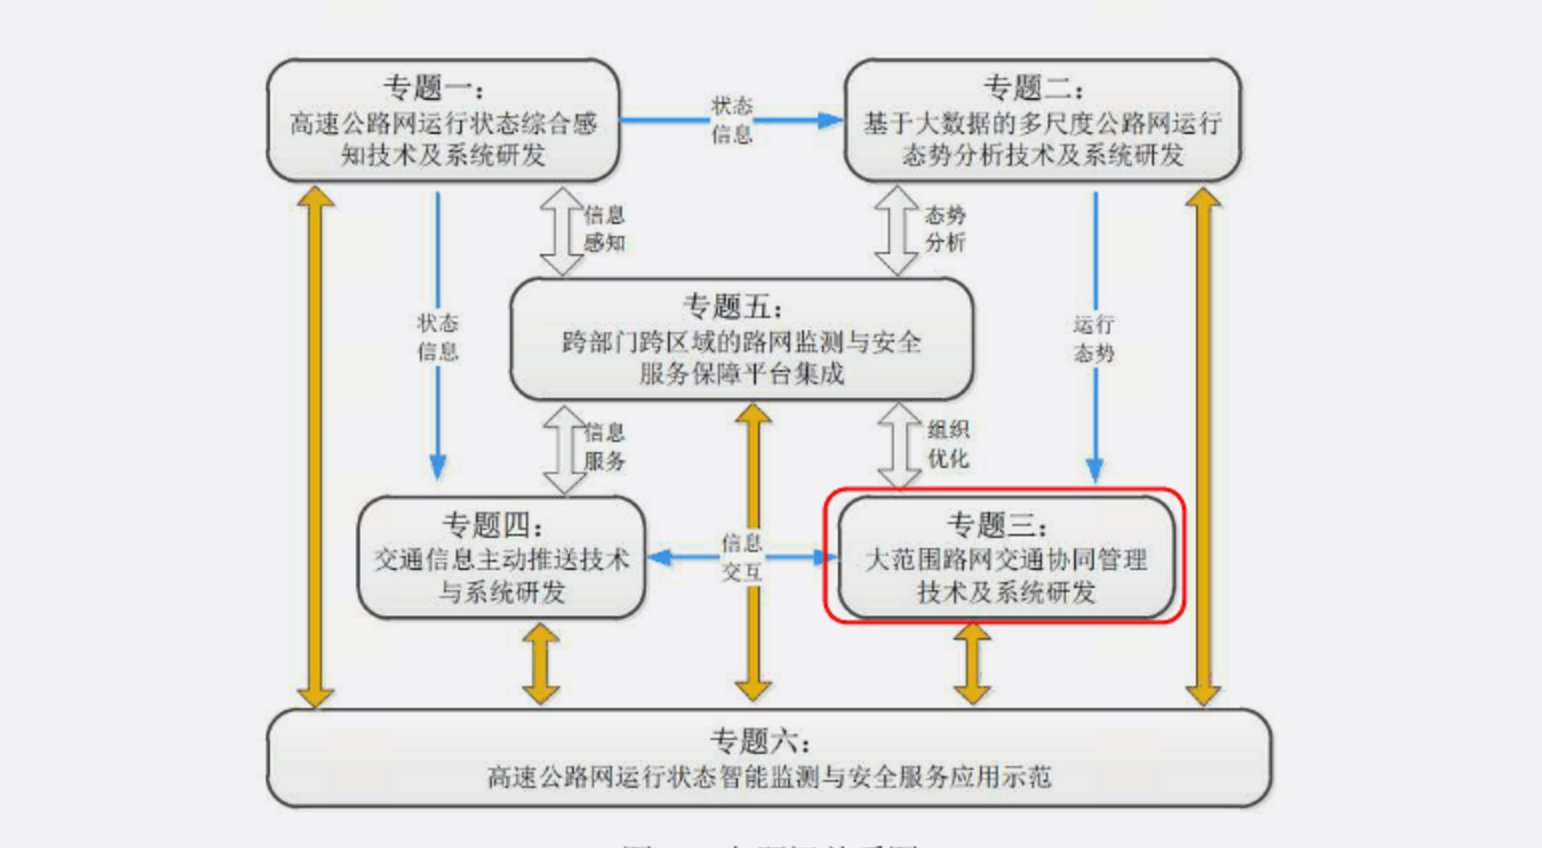
\includegraphics[width=4.4in]{picture/zhichengjihua}
							\caption{国家科技支撑计划}
							\label{zhichengjihua}
						\end{minipage}%\
				\end{figure}
图\ref{zhichengjihua}为项目专题间关系图,我们主要负责专题三:大范围路网交通协同管理技术以及系统研发。专题一主要研究高速公路的网络监测设施的部署问题,这些设施将用于改善路网运行状态以及获取路网运行数据;专题二主要用于分析和处理这些数据,将这些数据转化为流量、速度、密度和O-D信息。专题三负责提出决策模型,基于前面专题获取的数据,输出目前路网状态下最合理的绕行路线和限流建议;专题四负责研究如何设置设施,将这些建议分发出去;专题五和专题六负责将整个系统进行集成。可以看出,本课题中的专题一、专题三、专题四都和高速公路重要路段挖掘方法有关。专题一中的监测设施主要部署在重要路段中,优化监测效果;专题三中的决策模型可以基于路段的重要程度,策划导流决策;专题四中可以根据重要路段的分布信息,划定信息发布点,优化信息发布行为。





\section{研究内容}
    	本文从交通领域的诸多实际问题出发,研究高速公路关键路段挖掘问题。针对现有复杂网络关键路段挖掘技术的不足,提出以下两个研究思路:
    
		1)提出一种基于贪心算法的关键路段挖掘模型,并给出次模性证明。在高速路网上建设基础设施、部署警力,增加维护成本,都可以归类于对高速公路中路段的资源投放问题。本文提出关键路段挖掘模型,以每条路段都具有一定的损毁概率为基础,定义当路段获得投资后,损毁概率下降;结合路段损毁概率矩阵,计算用户的出行效率,最终获得高速公路的通行效率。文中分析了目标模型的性质,证明了模型的次模性,并给出了贪心求解步骤。

		2)提出一种基于复杂网络社群划分算法的关键路段挖掘模型。本文提出的关键路段挖掘模型,本质上可归类于概率规划问题,时间复杂度达指数级。在小范围路网中,模型计算时间较少,可以实现静态路网中关键路段的挖掘。但是在大范围路网中,算法的时间消耗会急剧增长,而且算法对于需要实时动态分析关键路段的需求无法满足。本文同时分析了以往复杂网络社群划分的局限性,给出一种结合高速公路的网络特性的社群划分方法。根据高速公路路段特性,结合模拟退火和变权算法,解决传统社群划分方法中的低分辨率问题\parencite{WeightPretreatment}和极端退化问题\parencite{WeightPretreatment},结合投资问题,在有限的误差下快速求解关键路段。

\section{研究意义}
		研究意义主要包括两个方面:

		1)应用实践价值:从应用的角度来看,随着我国高速公路网络规模的逐渐扩大,路网结构日益复杂,人们的出行需求逐年增加,高速公路遇到的挑战不断增加,高速公路的稳定越来越重要。高速公路监测设施不断完善,可以实时监测高速公路中的车流信息。本文结合高速公路的特性,解决传统关键路段挖掘方法中的不足,优化时间复杂度,使得模型可以在可承受时间复杂度内求解,最终实现静态、动态挖掘路网的关键路段。

		2)理论研究价值:本文提出的“面向高速公路的关键路段挖掘模型”具有一定的理论创新性。将一些高速公路建设上的具体问题抽象成一类基础问题,并给出一个可行解。传统高速公路关键路段研究,大多是研究高速公路的统计特性(如流量的大小,路段周围城市的重要程度,路段周围环境的变化等),本文利用数学模型描述各类高速公路现象,从宏观角度给出并求解一种具有普适性的高速公路关键路段挖掘模型。
		
\section{论文结构}
    第一章为绪论,介绍了本文的研究背景,提出了本文的研究内容。第二章
介绍了相关研究,主要介绍了高速公路关键路段研究、复杂网络关键路段研究的相关工作,结合交通问题的特点分析了现有方法的优势与不
足;同时对复杂网络社群划分方法及其相关研究进行了介绍,通过对现有社群划分方法的分类对比,分析了它们的优势与不足;第三章论述本
文的主要研究内容,提出了一种复杂网络关键路段挖掘模型,分析模型的贪心可解性,并给出了贪心解法与实验。第四章
提出了一种基于复杂网络社群划分的关键路段挖掘方法,给出了高效的优化算法和详
尽的理论分析,并在多个数据集下的进行了验证。第五章给出了本文实现的一个原型系统,并且已经在实际数据上运行。第六章给出了全文的总结与未来工作展望。


